%&program=xelatex
%&encoding=UTF-8 Unicode

\documentclass[12pt,oneside,a4paper,titlepage,final]{article}
\usepackage{fontspec}
\usepackage{indentfirst}
\usepackage{setspace}
\usepackage{graphicx}
\usepackage[czech]{babel}
\usepackage[pdfborder={0 0 0},pdfpagelabels=true,plainpages=false]{hyperref}
\usepackage[all]{hypcap}

\usepackage{amsmath}
\usepackage{amsthm}

\newtheoremstyle{note}{\parskip}{0pt}{}{\parindent}{\bfseries}{:}{.5em}{}
\theoremstyle{note}
\newtheorem*{warning}{Pozor}

% Better quotations
\renewcommand*{\uv}[1]{\quotedblbase #1\textquotedblleft}

% Metadata
\newcommand{\gettitle}{logdiag}
\newcommand{\getsubtitle}{Průvodce uživatele}
\newcommand{\getauthor}{Přemysl Janouch}
\newcommand{\getdate}{6. března 2011}

\hypersetup{pdftitle={\gettitle{} --- \getsubtitle},pdfauthor={\getauthor}}

\begin{document}

% Number the first pages with roman numerals
\renewcommand{\thepage}{\roman{page}}

% The title page has no header or footer at all
\thispagestyle{empty}

\begin{center}
	\doublespacing
	\textbf{\LARGE\gettitle}\\{\Large\getsubtitle}
	\par\getauthor
	\par\getdate
	\vfill
	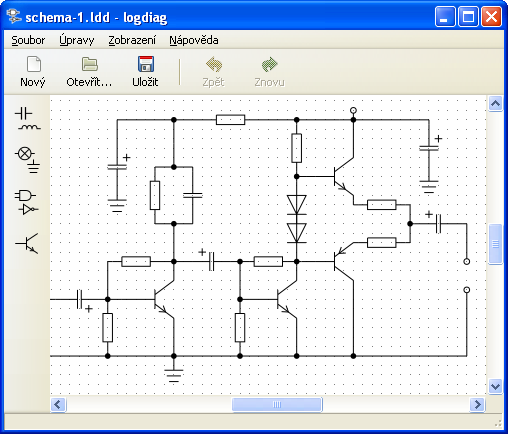
\includegraphics{logdiag-cs}
	\newpage
\end{center}

\tableofcontents
\newpage

% Number the real content with arabic numerals and show them in the footer
\renewcommand{\thepage}{\arabic{page}}
\setcounter{page}{1}

\section{Úvod}
Tento dokument vás má za účel provést po aplikaci a~pomoci vám se v~ní zorientovat. Popis úkonů se přednostně vztahuje na operační systém Microsoft Windows, do jisté míry je však platný i~pro jiné operační systémy.

\section{Získání aplikace}
Nejnovější verzi aplikace je možné stáhnout na následující webové adrese: \mbox{\url{http://github.com/pjanouch/logdiag}}.

\begin{figure}[ht]
	\centering
	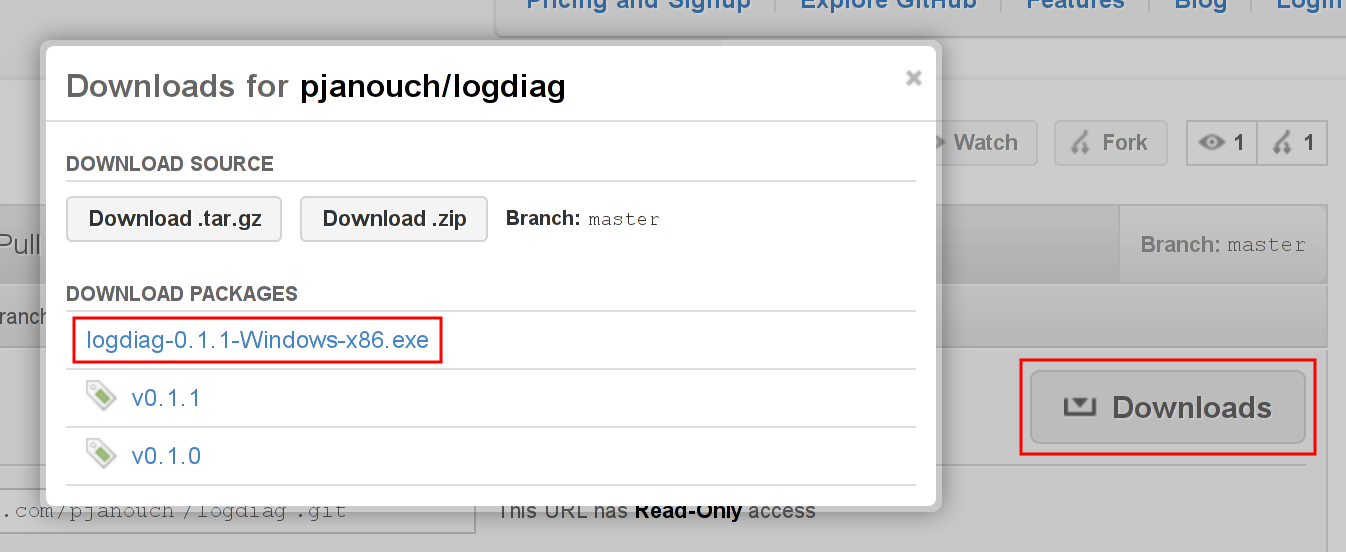
\includegraphics[width=\textwidth,keepaspectratio]{github}
	\caption{Nabídka pro stahování na githubu}
	\label{github-download}
\end{figure}

Až se ocitnete na githubu, vyhledejte po pravé straně tlačítko s~nápisem \uv{Downloads}, případně \uv{Soubory ke stažení}, a~klepněte na něj. Zobrazí se před vámi nabídka balíčků. Instalační soubor pro Microsoft Windows nese název ve stylu \uv{logdiag-\emph{verze}-Windows-x86.exe}.

\section{Instalace}
Proces instalace je velmi přímočarý. Po úvodní obrazovce je vyžadován souhlas s~licencí. Pokud nerozumíte anglicky, její stručné shrnutí zní, že aplikaci smíte v~nezměněné formě zcela volně používat a~redistribuovat, ale nejsou vám poskytovány žádné záruky. Následuje výběr složky, do které chcete aplikaci nainstalovat, a~složky pro umístění ve Start menu. V~případě, že nenastala žádná náhlá chyba, už jen stačí potvrdit úspěšnou instalaci.

\begin{warning}
	Pokud aplikaci instalujete do složky, kde se nachází již existující instalace, mohou nastat potíže. Ačkoliv je to možné, nepokoušejte se z~těch samých příčin instalovat ani více kopií vedle sebe. Nejdříve stávající instalaci odstraňte, například pomocí zástupce umístěného ve Start menu.
\end{warning}

\section{Operace s~objekty}
% TODO: Zkusit restrukturalizovat na:

% 4. Operace s objekty
%    4.1 Základní operace
%        4.1.1 Výběr
%        4.1.2 Přesun
%        4.1.3 Odstranění
%    4.2 Značky
%        4.2.1 Vložení
%        4.2.2 Otáčení
%    4.3 Spojení
%        4.3.1 Tvorba
%

Každý diagram je tvořen z~objektů, a~s~těmi se sdružují dále popsané operace. Budete-li chtít momentálně prováděnou operaci zrušit, můžete tak obvykle učinit stiskem klávesy Escape.

\subsection{Výběr objektů}
Jednotlivé objekty můžete vybírat levým kliknutím myší. Ty se v~reakci na to vyznačí červenou barvou. Chcete-li vybrat objektů více, držte během klikání stisknutou klávesu Shift.

\begin{figure}[ht]
	\centering
	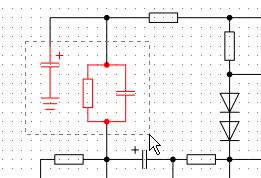
\includegraphics{select-objects}
	\caption{Výběr objektů v~oblasti}
	\label{select-objects}
\end{figure}

Alternativně můžete táhnout myší z~volné oblasti diagramu do prostoru, viz obrázek \ref{select-objects}. Vyberou se objekty obsažené ve vytvořeném obdélníku. Výběr lze zrušit klepnutím na prázdné místo.

\subsection{Přesun objektů}
Přesun objektů se provede tažením objektů myší na požadované místo. Pokud jsou tyto objekty součástí výběru, přesune se celý výběr. Ten lze též přesouvat pomocí kurzorových kláves.

\subsection{Odstranění objektů}
Objekty odstraníte stisknutím klávesy Delete, případně z~menu aplikace.

\subsection{Vložení značky}
\emph{Značky} představují nejdůležitější druh objektů. Do diagramu je vložíte výběrem z~nabídky značek umístěné po~levé straně hlavního okna aplikace, viz obrázek \ref{select-symbol}. Po kliknutí na vámi vybranou značku klikněte znovu do diagramu na místo, kde ji chcete umístit.

\begin{figure}[ht]
	\centering
	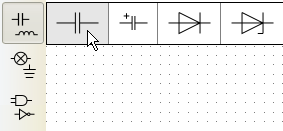
\includegraphics{select-symbol}
	\caption{Výběr značky z~nabídky}
	\label{select-symbol}
\end{figure}

\subsection{Otáčení značek}
Otočit značku vloženou do diagramu můžete přes pravé tlačítko myši.

\subsection{Propojení terminálů}
\emph{Terminálem} se nazývá bod určený pro tvorbu spojení mezi značkami nebo jinými spojeními. Abyste z~něj spojení vyvedli, nejdříve na něj najeďte kurzorem myši tak, aby se viditelně vyznačil kroužkem. Pak stiskněte levé tlačítko myši a~přetáhněte kurzor myši na místo, kde chcete, aby spojení končilo.

\begin{figure}[ht]
	\centering
	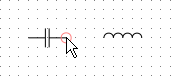
\includegraphics{create-connection-begin} \hspace{15pt} 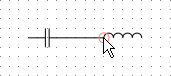
\includegraphics{create-connection-end}
	\caption{Propojení terminálů dvou značek}
	\label{create-connection}
\end{figure}

\section{Časté problémy}
\subsection{Nelze otevřít uložený diagram}
Při ukládání se ujistěte, že zadaný název souboru obsahuje příponu \uv{.ldd}. V~opačném případě se nezobrazí v~dialogu pro otevření diagramu. Pokud jste nějaký soubor již bez přípony uložili, napravíte to dodatečným přidáním přípony k~jeho názvu.

\subsection{Jak můžu diagram vytisknout?}
Současná verze aplikace není schopná přímo tisknout. Pro vytištění vytvořeného diagramu můžete klávesou PrintScreen sejmout snímek obrazovky, vložit jej například do aplikace Malování, oříznout požadovanou část a~vytisknout ji z~tohoto grafického editoru.

\subsection{Schází mi popisky}
Obdobně jako v~předchozím případě tato funkcionalita zatím neexistuje, ale je možné tento nedostatek obejít přes běžný grafický editor.

\end{document}


